\section{Research Goals And Significance }

\subsection{Detection of anchor amino acids in high resolution cryo-EM density maps }
We propose a Deep Learning based method for the detection of 
high confidence anchor amino acid residues in high resolution cryo-EM maps.
We focus on detection of  {\bf amino acid anchors} in the density map, namely having knowledge of even a relatively small number of amino acids, whose identity and location has been established with high confidence.
Reliable prior detection of amino acid anchors can be used to guide the various de-novo modeling methods, as well as serve as a starting point for the development of novel methods.
In particular, it could lead to the development of novel techniques, which do not require prior segmentation of the EM density map.
The lack of sufficient experimental data required for  the training stage is the main expected pitfall. 
We propose two different approaches to cope with the shortage of experimental data.

 
\paragraph{Integrating X-ray crystallography data with cryo-EM for structure determination}.

X-ray crystallography is an invaluable tool for revealing the  three-dimensional structure of molecules. 
Contemporary online databases: CSD ( \url{http://www.ccdc.cam.ac.uk}) ,PDB (\url{http:// www.rcsb.org/pdb}, and  PDBe (\url{http://www.ebi.ac.uk/pdbe/node/1}) contain more than 100,000 biological macromolecules.


While having the same form of a 3D matrix of density values, Xray crystallography data differs from cryo EM data in the conditional distribution of the outputs given the inputs.
The problem is known as \textit{dataset shift}, \cite{Quinonero-Candela2010 }.
This is due to different principles of cryo-EM and X-ray crystallography experiments, from specimen preparation to data processing, (see Figure ~\ref{f:em_cryst} and \cite{Zanotti2016}, \cite{Zeng2018},\cite{Wang2017},\cite{Venien-Bryan2017} for details).

The proposed algorithm is to train a CNN on large amount of X-ray data ( \textit{source domain}) with the existing cryo-EM data (\textit{target domain}) .
A \textbf{domain adaptation} procedure will be applied to compensate for  the difference  between the source and the target domains. 


The presented  algorithm contains a novel approach  to  cryo-EM and X-ray processing in which both data types complement each other in the task of atomic structure determination.
Running the algorithm on new experimental data will reveal structural properties at high precision, which is crucial for revealing the functionality and for drug design.



\begin{figure}[!ht]

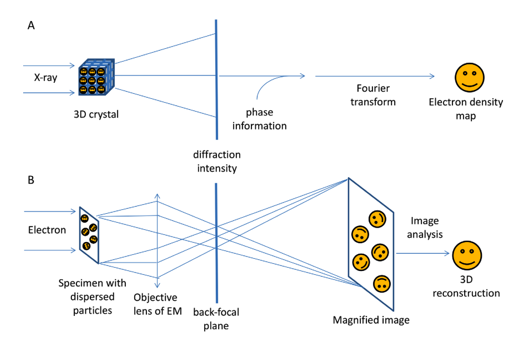
\includegraphics[width=0.95\textwidth]{pics/em_cryst}
\caption{Technical difference between X-ray crystallography and single particle cryo-EM. }\label{f:em_cryst}
\end{figure}

\begin{figure}[!ht]

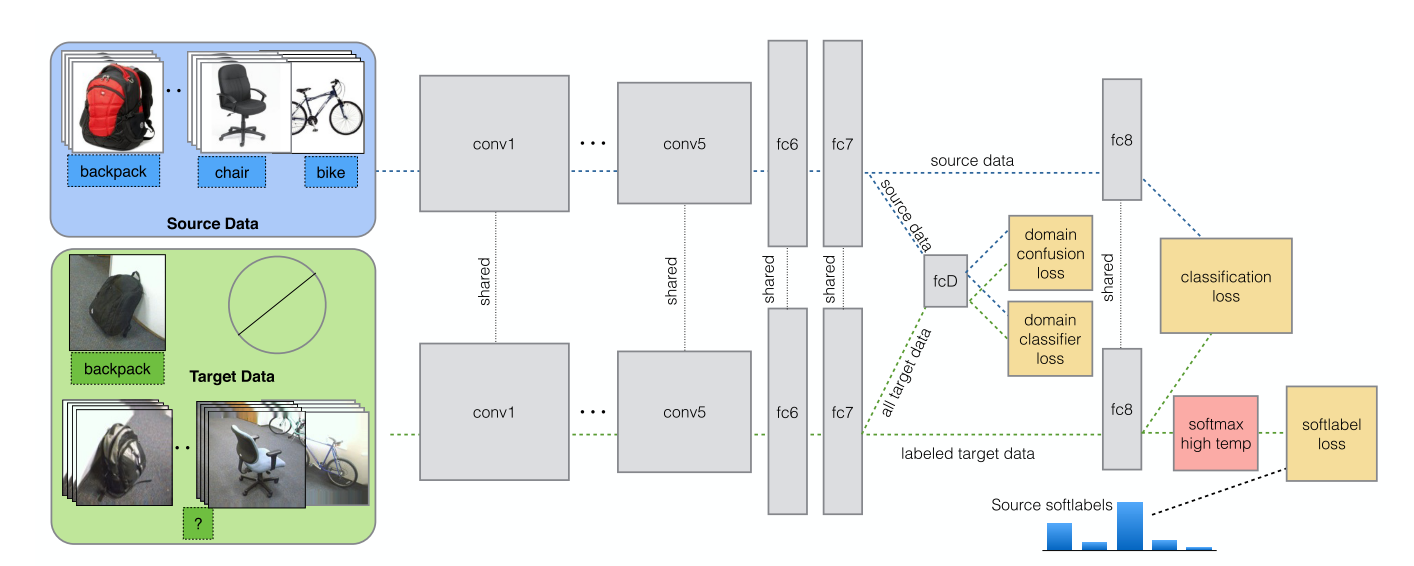
\includegraphics[width=0.95\textwidth]{pics/dom_conf_1}
\caption{Deep Domain Confusion Architecture }\label{f:dom_conf_1}
\end{figure}



\subsection{Simulating cryo-EM maps using Generative Adversarial Network}
Our previous work on the AAnchor algorithm \cite{Rozanov2018AAnchor:Maps}, showed that augmenting a training dataset by  synthetic data improves a classification CNN performance. 
Contemporary models for generating   synthetic cryo EM maps from atomic structure are incapable to generate realistic data.
We propose to use Generative Adversarial Networks  with Variation AutoEncoder (VAE-GAN) to create cryo-EM maps which are indistinguishable from experimental ones.
GANs  and VAEs are proven deep learning techinques for generating 2D and 3D images.
Reliable cryo EM map simulation is of great significance for the protein structural modelling task. 
In addition to augmenting the training dataset as in our case, such simulation is capable of improving performance of template matching based modelling methods: PowerFit \cite{C.P.vanZundert2015}, MultiFit \cite{Tjioe2011}, EMatch \cite{Dror2006}, and others. 



\subsection{Annotating Secondary Structure in Medium Resolution ($4 -6$ {{\AA} } ) cryo-EM maps}

We propose a Deep Learning based method for the detection  of Secondary Structure Elements (SSE) in medium resolution cryo-EM map.
Locating SSEs (helices, beta-strands) is of high importance to protein modelling and number of methods have been developed for the task.
One group of the developed  methods uses image  processing tools, for locating cylinder-like (helices) and plane (beta-sheets) structures, \cite{Baker2007a},  \cite{Jiang2001}, \cite{Rusu2012}, \cite{Yu2008}.
Another family of SSE detections methods uses ML approach \cite{Ma2012RENNSH:Maps} \cite{Si2012a} including  deep CNNs \cite{Velankar2012}, \cite{Li2016},\cite{Ma2003}, \cite{Mostosi2019AutomatedNetworks}.


While the above mentioned methods relied solely on structural features, we propose an \textbf{integrative} method  which 
incorporates protein sequence information as well.
The query protein sequences are used to search for homologs with known structure.
A realistic cryo-EM simulation will be used to create a dataset from these homologous structures.
The new dataset should have a similar features distribution as the query map.
The created synthetic dataset will be used for fine tunnig of the detection CNN.

\subsection{ Detection of binding sites (BSs)  in medium resolution ($4 -6 ${{\AA} } ) cryo-EM density maps}
Whilst de-novo protein modeling from a median resolution map remains an unresolved problem, we focus on locating BSs.  
Our task is to mark voxels in the cryoEM map which belong to a protein-protein interface or  a protein binding site.
Since  BSs dictate the molecular function, they are usually more evolutionary conserved and tolerate less flexibility than less functionally important parts of a protein structure. 
A deep learning approach will benefit from both of the above mentioned  properties.
Evolutionary conservation leads to a greater amount of similar structures in existing databases. 
Due to the limited flexibility, structures under search should be similar or nearly similar to those in a database. 
Locating  BSs is an important step towards full atomic structure determination, since it provides information about protein tertiary structure and separation to domains.
From a biological point of view  BSs are key to understanding protein functionality
\paragraph{Integrative algorithm for finding conserved structures in cryo-EM maps.}
The existing vast amount of data about conserved structures, is hard to utilize, since it  belongs to different domains.
Resolved protein structures are represented as lists of atom positions.
Results of cryo-EM experiments are given in a form of a 3D matrix of electron density.
Sequence data is represented as a list of chains, where each chain is an ordered sequence from an alphabet of twenty letters.  
To address the challenge of utilizing all three types of data, we suggest a deep learning algorithm architecture which combines a standard Convolutional Neural Network with Generative Adversarial Network, Transfer Learning and Multiple Sequence Alignment.
